%%%%%%%%%%%%%%%%%%%%%%%%%%%%%%%%%%%%%%%%%
% fphw Assignment
% LaTeX Template
% Version 1.0 (27/04/2019)
%
% This template originates from:
% https://www.LaTeXTemplates.com
%
% Authors:
% Class by Felipe Portales-Oliva (f.portales.oliva@gmail.com) with template 
% content and modifications by Vel (vel@LaTeXTemplates.com)
%
% Template (this file) License:
% CC BY-NC-SA 3.0 (http://creativecommons.org/licenses/by-nc-sa/3.0/)
%
%%%%%%%%%%%%%%%%%%%%%%%%%%%%%%%%%%%%%%%%%

%----------------------------------------------------------------------------------------
%	PACKAGES AND OTHER DOCUMENT CONFIGURATIONS
%----------------------------------------------------------------------------------------

\documentclass[
	10pt, % Default font size, values between 10pt-12pt are allowed
	%letterpaper, % Uncomment for US letter paper size
	spanish % Uncomment for Spanish
]{fphw}

% Template-specific packages
\usepackage[utf8]{inputenc} % Required for inputting international characters
\usepackage[T1]{fontenc} % Output font encoding for international characters
\usepackage{mathpazo} % Use the Palatino font
\usepackage{graphicx} % Required for including images
\usepackage{booktabs} % Required for better horizontal rules in tables
\usepackage{listings} % Required for insertion of code
\usepackage{enumerate} % To modify the enumerate environment
\usepackage[spanish, es-tabla]{babel}
\usepackage{spverbatim}

%----------------------------------------------------------------------------------------
%	ASSIGNMENT INFORMATION
%----------------------------------------------------------------------------------------

\title{Reporte Práctica \#2} % Assignment title

\author{César Augusto Farrera Ortega (311617670) \\ Karem Ramos Calpulalpan (314068583)} % Students name

\date{02/03/2020} % Due date

\institute{UNAM \\ Facultad de Ciencias} % Institute or school name

\class{Fundamentos de bases de datos} % Course or class name

\professor{Gerardo Avilés} % Professor or teacher in charge of the assignment

%----------------------------------------------------------------------------------------

\begin{document}

\maketitle % Output the assignment title, created automatically using the information in the custom commands above

%----------------------------------------------------------------------------------------
%	ASSIGNMENT CONTENT
%----------------------------------------------------------------------------------------

\section*{Análisis de requerimientos}


\subsection*{Enumeración de los requerimientos candidato}
\begin{enumerate}
	\item Almacenar información sobre los chofores.
	\item Almacenar información sobre los dueños del taxi.
	\item Almacenar información sobre los taxis, dentro de la asociación.
	\item Capturar información sobre choferes, dueños de taxis y taxis.
	\item Consultar información sobre choferes, dueños de taxis y taxis.
	\item Editar información sobre choferes, dueños de taxis y taxis..
	\item Eliminar información sobre choferes, dueños de taxis y taxis..
	\item Guardar informacion sobre choferes, dueños de taxis y taxis.
	\item Leer información sobre choferes, dueños de taxis y taxis.
\end{enumerate}
\subsection*{Comprensión del contexto del sistema}
Digrama casos de uso.

\begin{figure}[h]
	\centering
	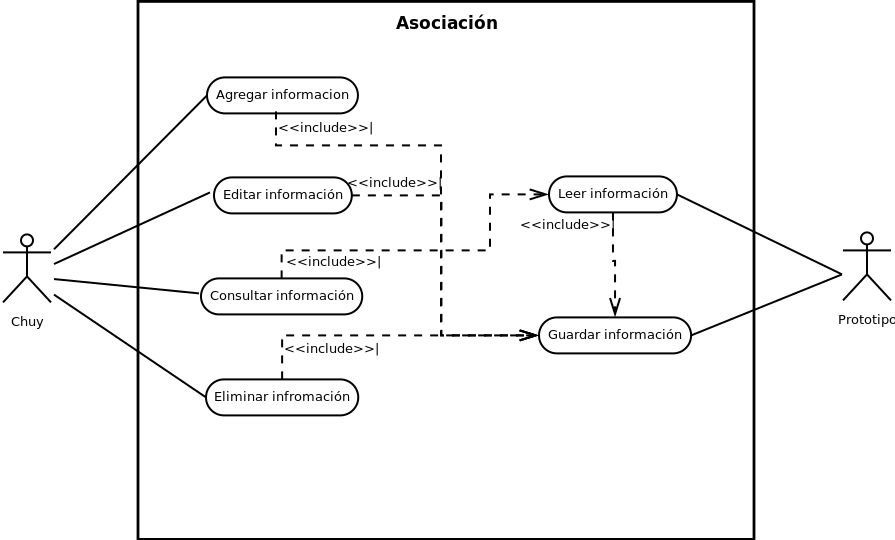
\includegraphics[scale=0.4]{DiagramaCasosDeUsoAsociacion.png}
\end{figure}
\subsection*{Captura de requerimientos funcionales}
\begin{enumerate}
	\item El prototipo debe almacenar la información  personal de choferes, dueños de taxis y taxis.
	\item El prototipo debe permitir capturar, consultar, editar y eliminar información personal de choferes, dueños y taxis, 		teniendo en cuenta que la relación existe entre las tres entidades.
	\item La información capturada se tiene que persistir, por lo que el sistema debe guardar y leer la información en 				archivos .CVS.
\end{enumerate}
\subsection*{Captura de requerimientos no funcionales}
\begin{enumerate}
	\item La información almacenada debe estar abstraida de manera eficiente, pues se espera posteriormente crear una base de 
	datos.
	\item Los archivos deben estar organizados correctamente, para un menejo eficaz de ello. 
	\item El prototipo debe abstraer datos personales de choferes, dueños de taxis y taxis, incluyendo fecha de inicio como 		asociado, para un uso coherente de la información.
	\item Idenficar la información del taxi, para saber que es funcional para la asociación.	
\end{enumerate}
%----------------------------------------------------------------------------------------

\section*{Preguntas}

\begin{problem}
Describe cinco diferencias entre almacenar la información utilizando un sistema de archivos a almacenarla utilizando una base
de datos. Deberás describir que es mas conveniente utilizar
\end{problem}

\subsection*{Respuesta}

\begin{enumerate}
	\item {\bf{Relación entre datos}}. En un sitema de archivos, los archivos pueden tener relación entre sí, pero no es fácil de vizualizar esa relación, en una base de datos las relaciones se dan por tablas, creando una fácil relación entre datos. Si se quisiera una vizualización práctica de datos, es más recomandable una base de datos.
	\item {\bf{Acceso a datos}}. El acceso a la información para consulta o modificación de los datos no es tan práctica, cuando manejamos la información en un sistema de archivos, además que es fácil tener información duplicada. En una base de datos, gracias a su diseño, no pueden existir dos tablas con el mismo nombre ni registro; las llaves primarias restringen la integridad de los datos. Si manejamos muchos datos, claramente sería más práctico usar una base de datos, pues la situación de datos duplicados nos causarían conflicto en ciertas acciones del sistema. 
	\item {\bf{Tipos de datos}}. En una base de datos, podemos guardar la información en múlitples tipos de datos, en cambio, cuando usamos sistemas de archivos, para los distintos tipos de datos sólo usamos texto. 
	Si los datos que vamos a maniúlar osn de distintos tipos, deberíamos optar por usar una base datos, por la gran variedad que nos ofrece, si supieramos que sólo tendremos un tipo de datos siempre, podría ser más práctico usar el sistema de archivos.
	\item {\bf{Almacenamiento de datos}}. Cuando manejamos la información en sistemas de archivos, los datos estarán dispersos en varios archivos y varios formatos, porque guardar los datos en archivos no restringe un formato en especifico. En una base de datos, los datos se guardan siguiendo un formato en tablas, teniendo un formato más natural. Sería más conveniente las beses de datos, ya que el cómo guardar nuestros datos, influirá mucho a la ahora de busqueda de datos, si el formato en que lo guardamos no es el mismo será muy difícil encontrar un dato.
	\item {\bf{Seguridad de información}}. En una base de datos se puede definir las personas que tienen autorización para acceder a la información o incluso determinar que porción de información puede ver cada tipo de usuario. En un sistema de archivos no, el acceso no es restringido. Si manejamos datos importantes o personables sería desable usar una base de datos, para que esa información no se use de forma contraproducente.    	
\end{enumerate}

%----------------------------------------------------------------------------------------

\begin{thebibliography}{1}
  		\bibitem {} S.a., "Qué es un modelo de bases de datos", \underline{Lucidchart}, $<$https://www.lucidchart.com/pages/es/que-es-un-modelo-de-base-de-datos$>$, Domingo 1 de marzo del 2020, 14:14 hrs.
  		\bibitem {} S.a., "Sistemas de Bases de Datos vs Sistemas de Archivos", \underline{Fundamentos de BDs y algo más…}, $<$https://uvfdatabases.wordpress.com/2009/02/02/sistemas-de-bases-de-datos-vs-sistemas-de-archivos/$>$, Domingo 1 de marzo del 2020, 14:33 hrs.
  		\bibitem {} S.a., "Sistemas de bases de datos frente a los sistemas de archivos" \underline{Currículos en TIC exploratorios}, $<$http://contenidos.sucerman.com/nivel2/web1/unidad1/leccion2.html$>$, Domingo 1 de marzo del 2020, 15:16 hrs.
  		
\end{thebibliography}

\end{document}
